\documentclass[11pt]{article}
\usepackage{amsmath, amssymb}
\usepackage[margin=1in]{geometry}
\usepackage{enumitem}
\usepackage{graphicx}
\setlength{\parindent}{0pt}
\setlength{\parskip}{6pt}

\title{Insights from \texttt{synheart\_har\_pipeline}\\[2pt]
\large the 1D-CNN baseline (Synheart Kinematics)}
\date{}

\begin{document}
\maketitle

Short notes on the CNN pipeline. This is a much stronger baseline than the
starter: it reads the raw signals with a 1D-CNN (no $561$ features), uses
\textbf{LOSO} cross-validation, adds \textbf{SO(3) orientation augmentation},
exports to ONNX for on-device use, and keeps all six classes. Credit where due ---
the orientation instinct is the right one. The notes below are the gaps.

\section{The augmentation fights its own posture feature}
The three static postures --- sitting, standing, lying --- carry almost no motion:
the body-acceleration motion $\mathrm{std}(\lVert \mathbf{a}_{\text{body}}\rVert)$
is $\approx 0.011\text{--}0.016$ g for all three and fully overlapping
(Fig.~\ref{fig:pipe}, right). The only thing that separates them is
\texttt{gravity\_mean} --- the direction of gravity in the phone frame --- which
alone reaches $85.2\%$ on the three (Fig.~\ref{fig:pipe}, left).

But \texttt{gravity\_mean} is orientation-specific, and the SO(3) augmentation
rotates it over the whole sphere. After a random rotation the same cue drops to
$33.6\%$, i.e.\ chance ($\approx 34\%$). So the augmentation that buys orientation
robustness also \textbf{erases the only cue for the static postures}. You cannot
have full rotation invariance \emph{and} gravity-based posture from the same
input. The notebook presents augmentation as a pure gain; the cost to
sitting/standing/lying is never measured.

\section{Rotation robustness is never actually tested}
The whole pitch is ``orientation-robust,'' but augmentation is applied only to the
\emph{training} set and the model is evaluated on the original waist-fixed test
subjects. There is no rotated-test evaluation, so the headline claim is never
demonstrated on held-out data.

\section{LOSO and the final test number are not comparable}
LOSO ($30$ folds) is run \emph{without} augmentation, while the final reported test
accuracy is a single $70/10/20$ subject split \emph{with} augmentation. There is no
LOSO-with-augmentation, so the real effect of augmentation on a new person is never
shown --- two different protocols are reported side by side.

\section{Heavy for the brief}
The model is a $\sim 344$K-parameter CNN that needs training, a GPU, and an ONNX
runtime. The assignment asks for ``very lightweight, no thousands of features,
on-device.'' A CNN is the heavy end of that scale compared with a few-feature
deterministic rule --- a real engineering trade-off that is not discussed.

\section{Takeaway}
The pipeline is on the right track (raw signals, LOSO, augmentation), but it runs
into the same wall our work identifies: \textbf{motion is orientation-proof,
posture is not}. Forcing rotation invariance throws away the gravity direction that
the static postures depend on. That is why posture (sitting vs standing vs lying)
belongs to a separate gravity-aware stage, not to a fully rotation-invariant model.

\begin{figure}[h]
\centering
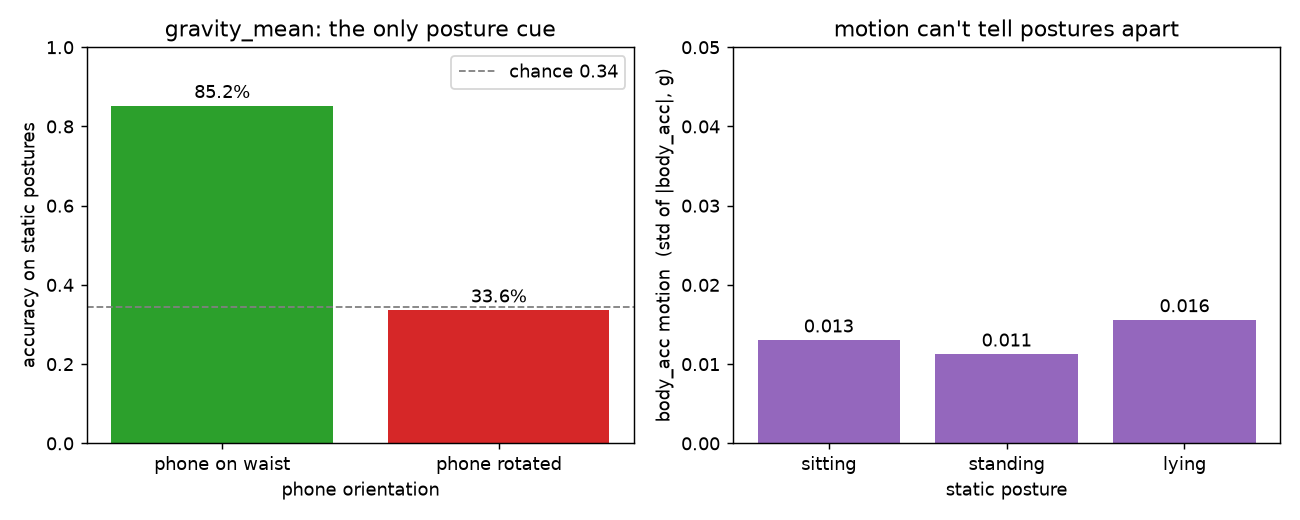
\includegraphics[width=\textwidth]{figs/fig_pipeline.png}
\caption{Left: \texttt{gravity\_mean} separates the three static postures at
$85.2\%$ on the waist data, but collapses to chance ($33.6\%$) once the phone is
rotated --- which is exactly what the SO(3) augmentation does. Right: body-motion
is tiny and overlapping for all three static postures, so motion alone cannot
separate them.}
\label{fig:pipe}
\end{figure}

\section{The other side of the map: the walk types}
For completeness, the dynamic classes (walking, ascending, descending) are the
mirror image --- they are a \emph{motion} question, not a gravity one. Using only
orientation-proof motion features from $\lVert\mathbf{a}_{\text{body}}\rVert$
(intensity and cadence), the three separate at $55.7\%$ (chance $35.8\%$):
descending stands out (harder impact, faster cadence $\approx 3$ Hz) while walking
and ascending overlap (Fig.~\ref{fig:walk}). The separation is partial and uses
\textbf{no gravity at all}. This confirms the division of labour: activity and
walk-type live on the orientation-proof motion side, posture lives on the
gravity side --- and only the latter breaks under rotation.

\begin{figure}[h]
\centering
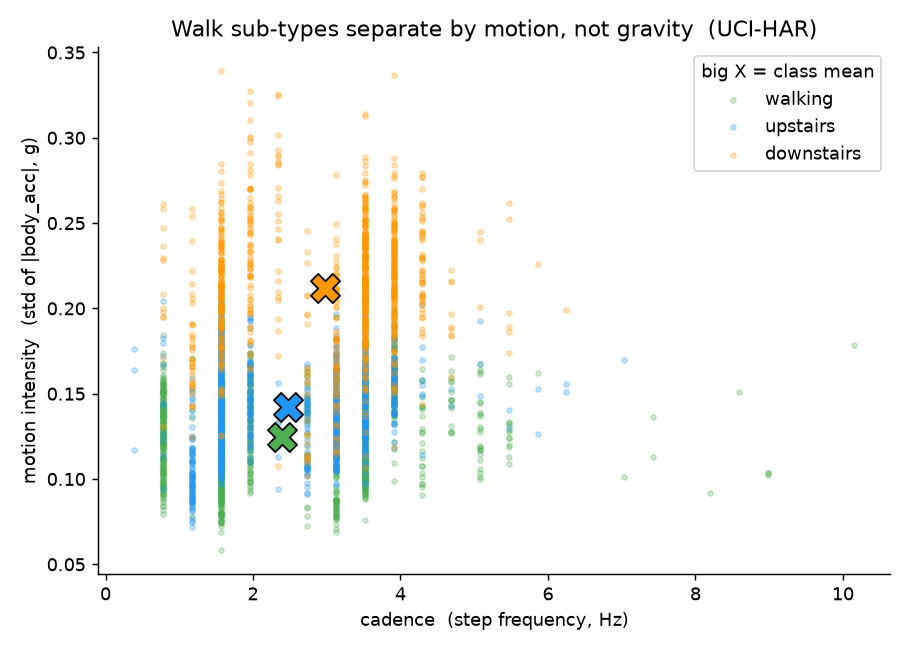
\includegraphics[width=0.72\textwidth]{figs/fig_walktypes.png}
\caption{The three walk types in orientation-proof motion space (UCI-HAR).
Descending separates by higher intensity and cadence; walking and ascending
overlap. No gravity direction is used, so this view is unchanged by phone
rotation.}
\label{fig:walk}
\end{figure}

\end{document}
